\section{}
Consider the pivot of unit thickness subject to force $P$ per unit thickness at its vertex (Figure \ref{fig:Q3ProblemDiagram}).
Determine the maximum values of $\sigma_x$ and $\tau_{xy}$ on a plane a distance $L$ from the apex through the use of $\sigma_r$
given by Eq. (3.43) and the formulas of the elementary theory. Take $\alpha = 30^\circ$.
\begin{figure}[h]
    \centering
    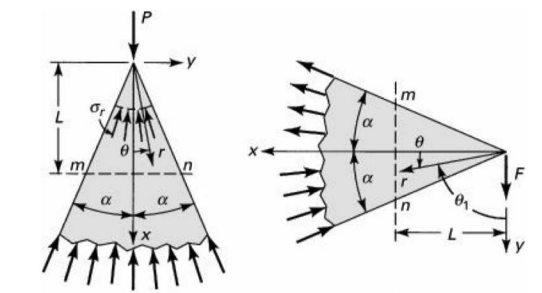
\includegraphics[width=0.3\linewidth]{Questions/Figures/Q3ProblemDiagram.png}
    \caption{Problem diagram for Question 3.}
    \label{fig:Q3ProblemDiagram}
\end{figure}
%notes
% \subsection*{Stress Concentrations}
% Wedge of unit thickness, under load $P$, and angle $\alpha$,
% \begin{gather*}
%     \sigma_{r} = - \frac{P \cos{\theta}}{r(\alpha + \frac{1}{2}\sin{2\alpha})},\quad \sigma_{\theta} = 0, \quad \tau_{r\theta} = 0\\
%     \sigma_{x} = \sigma_{r} \cos^2{\theta} = - \frac{P \cos^4{\theta}}{L(\alpha + \frac{1}{2}\sin{2\alpha})} \\
%     (\sigma_{x})_{\text{elem}} = - \frac{P}{2L\tan{\alpha}}
% \end{gather*}
% Note that the normal stress is maximum at $\theta = 0$ and minimum at $\theta = \alpha$

From the textbook the maximum stress occurs at $\theta = 0$. $\alpha = 30^\circ = \frac{\pi}{6}$
\begin{align*}
    (\sigma_{x})_{\text{elast}} &= - \frac{P}{L(\alpha + \frac{1}{2}\sin{2\alpha})} \\
    &= -\frac{P}{L(\pi/6 + \frac{1}{2}\sin{\pi/3})} \\
    &= \boxed{-\frac{P}{0.9566L}}
\end{align*}
Using elementary theory,
\begin{align*}
    (\sigma_{x})_{\text{elem}} &= - \frac{P}{A} = - \frac{P}{2 L \tan{\alpha}} \\
    &= - \frac{P}{2 L \tan{\pi/6}} \\
    &= \boxed{-\frac{P}{1.1547L}}
\end{align*}
From the textbook,
\begin{align*}
    (\tau_{xy})_{\text{elast}} &= \frac{P\sin\theta \cos\theta}L(\alpha + \frac{1}{2}\sin{2\alpha}) \\
\end{align*}
Since $\alpha \geq 30^\circ$, the maximum shear stress occurs at $\theta = 30^\circ$.
\begin{align*}
    (\tau_{xy})_{\text{elast}} &= \frac{P\sin\theta \cos^3\theta}{L(\alpha + \frac{1}{2}\sin{2\alpha})} \\
    &= \frac{P\sin(30^\circ) \cos^3(30^\circ)}{L(\pi/6 + \frac{1}{2}\sin{\pi/3})} \\
    &= \frac{0.324759526419P}{0.956611477491L} \\
    &= \frac{0.3395P}{L}\\
    &= \boxed{\frac{P}{2.946L}}
\end{align*}
From elementary theory,
\begin{equation*}
    (\tau_{xy})_{\text{elem}} = \frac{Tr}{J} = \boxed{0}
\end{equation*}